%2942
%22行目,33行目,48行目要確認
\newpage
\section{質問フォーム}

わからないこと、質問したいことがあれば質問フォームから質問しよう!

質問フォームでは、授業でわからなかったことや確認(かくにん)したいことなどをホームページを通して質問できます。たくさん質問してわからないことを解決しよう。

1.
ブラウザで\textbf{授業で使うホームページリスト}を開こう。

\textbf{授業で使うホームページリスト}は/home/ユーザー名/01フォルダの中のlinks.htmlです

リストの4番目の子ども\textbf{IT未来塾質問フォーム}をクリックして開いてください(Figure~\ref{fig:prog_menu})。


\begin{description}
    \item \textgt{\bf スマートフォン等からの場合は\url{https://bit.ly/2NHiVgi}を開いてください。}
\end{description}

% ここからコメントアウトだった
\begin{figure}[H]
    \begin{center}
      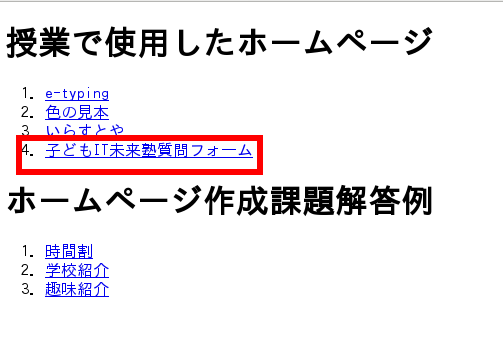
\includegraphics[width=11.231cm,height=7.613cm]{text04-img/textbook-img245.png}
      \caption{ホームページリストより質問フォームを開く}
    \end{center}
    \label{fig:prog_menu}
\end{figure}

2.
% 質問フォーム(Figure~\ref{seq:fig:prog_menu})が表示されます
質問フォーム(Figure~\ref{fig:prog_menu})が表示されます
\begin{figure}[H]
    \begin{center}
      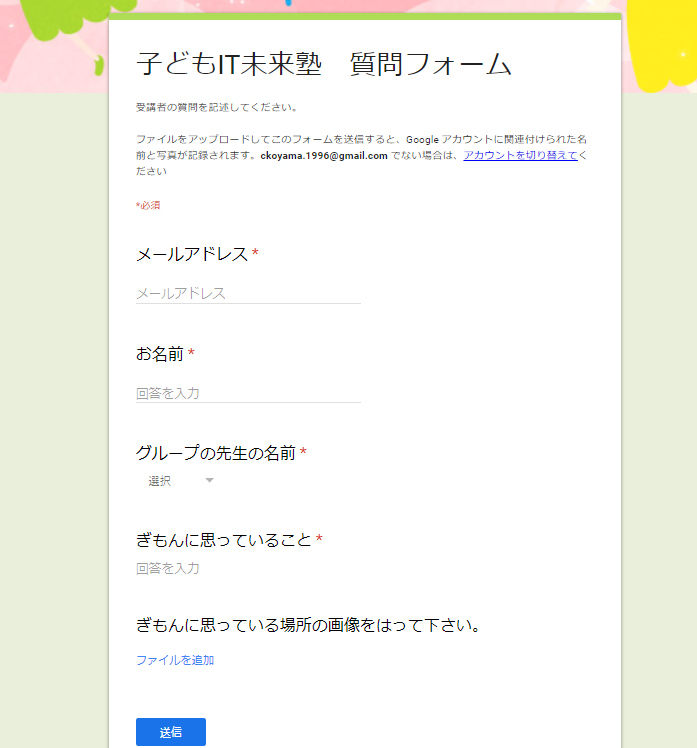
\includegraphics[width=13.263cm,height=14.233cm]{text04-img/textbook-img246.png}
      \caption{質問フォーム}
    \end{center}
    \label{fig:prog_menu}
\end{figure}

メールアドレス、お名前、グループの先生の名前、ぎもんに思っていることを入力します。必要に応じて、ぎもんに思っている場所の画像を追加してください。

\begin{description}
    \item \textgt{\bf 送信\textmd{を押すと質問ができます。Figure~\ref{fig:prog_menu2}の画面が出たら質問は完了です。}}
\end{description}


\begin{figure}[H]
    \begin{center}
      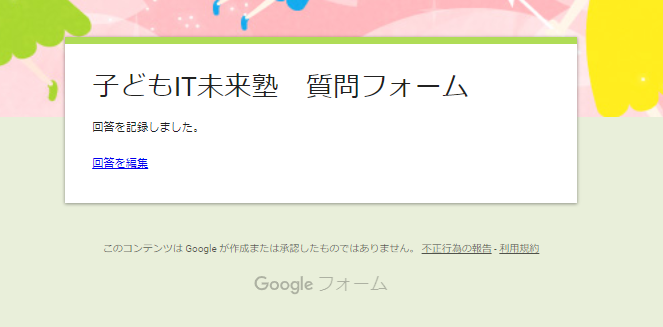
\includegraphics[width=8.871cm,height=4.374cm]{text04-img/textbook-img247.png}
      \caption{質問送信画面}
    \end{center}
    \label{fig:prog_menu2}
\end{figure}

メールアドレスのらんに入力したアドレスへグループの先生から回答メールがきます。
メールが来るまで、しばらくお待ちください。数日かかる場合があります。





